\documentclass[first=purple,second=dgreen,logo=blueexc]{aaltoslides}

\usepackage[latin9]{inputenc}
\usepackage[T1]{fontenc}
\usepackage{graphicx}
\usepackage{amsfonts,amssymb,amsbsy,amsmath}
\usepackage{tikz}
\usepackage{url}
\usepackage{lastpage}
\usepackage{subfig}

\title{non-static object capture using multi-view stereo video}

\author{Konsta H�ltt�}
\institute{AS-0.3100 seminar presentation\\
konsta.holtta@aalto.fi}

\aaltofootertext{MVS non-static capture}{Apr 25, 2014}{\arabic{page}/\pageref{LastPage}\ }

\date{Apr 25, 2014} % \today}

\newcommand{\kuva}[2]{\begin{figure}[h]
\includegraphics[width=#1\textwidth]{gfx/#2}
\end{figure}}

\newcommand{\simplefig}[4]{%
	\begin{figure}[#1]\begin{center}
		#2
		%\caption{#4}
		%\label{#3}
	\end{center}\end{figure}
}
% \simplegfx{pos-specifier}{width}{filename-and-labelname}{caption}
\newcommand{\simplegfx}[4]{%
	\simplefig{#1}{\includegraphics[width=#2]{gfx/#3}}{fig:#3}{#4}
}

\begin{document}

%%%%%%%%%%%%%%%%%%%%%%%%%%%%%%%%%%%%%%%%%%%%%%%%%%%%%%%%%%%%%%%%%%%%%%%%%%%%%%%%%%%%%%%%%%%%%

\aaltotitleframe

%%%%%%%%%%%%%%%%%%%%%%%%%%%%%%%%%%%%%%%%%%%%%%%%%%%%%%%%%%%%%%%%%%%%%%%%%%%%%%%%%%%%%%%%%%%%%

\begin{frame}{Intro}
\begin{itemize}
	\item Non-static / dynamic: moving or morphing over time
	\item $\Rightarrow$ video, maybe not just a simple object
	\item object: some target of interest in front of a camera
	\item capture: encode the object's visual properties to a computer \begin{itemize}
		\item geometry: 3d surface structure
		\item texture: (diffuse) color
		\end{itemize}
	\item multi-view stereo: recover 3D from photographs
	\item video: a sequence of frames
\end{itemize}
this presentation reviews the parts of the capture pipeline
\end{frame}

%%%%%%%%%%%%%%%%%%%%%%%%%%%%%%%%%%%%%%%%%%%%%%%%%%%%%%%%%%%%%%%%%%%%%%%%%%%%%%%%%%%%%%%%%%%%%

\begin{frame}{Contents}
\begin{itemize}
	\item Motivation
	\item Imaging basics
	\item Stereo reconstruction
	\item Multi-view stereo
	\item Motion specifics
	\item Post processing
	\item Conclusion
\end{itemize}
%\kuva{0.6}{ankka.jpg}
\end{frame}

%%%%%%%%%%%%%%%%%%%%%%%%%%%%%%%%%%%%%%%%%%%%%%%%%%%%%%%%%%%%%%%%%%%%%%%%%%%%%%%%%%%%%%%%%%%%%

\begin{frame}{Motivation}
\begin{itemize}
	\item applications in mapping, object replication, entertainment, cultural heritage, medical, crime scenes, ...
	\item most visible in modern movies and video games
	\item facial expressions; motion/surface capture
	\item relatively cheap hardware
\end{itemize}
%\kuva{0.6}{ankka.jpg}
\end{frame}

%%%%%%%%%%%%%%%%%%%%%%%%%%%%%%%%%%%%%%%%%%%%%%%%%%%%%%%%%%%%%%%%%%%%%%%%%%%%%%%%%%%%%%%%%%%%%

\begin{frame}{Pipeline}
\begin{itemize}
\item Calibration: capture camera rig parameters
\item Imaging: Record the object movement as series of images
\item 3D Reconstruction \begin{itemize}
  \item stereo matching, rectification
  \item feature tracking
  \item triangulation, point clouds \end{itemize}
\item Meshing: from point clouds to 3D models
\item Rendering: draw the model on a computer screen (or use in other ways)
\end{itemize}
%\kuva{0.6}{ankka.jpg}
\end{frame}

%%%%%%%%%%%%%%%%%%%%%%%%%%%%%%%%%%%%%%%%%%%%%%%%%%%%%%%%%%%%%%%%%%%%%%%%%%%%%%%%%%%%%%%%%%%%%

\begin{frame}{Cameras}
%\simplegfx{h}{0.6\textwidth}{pinhole-camera}
%{Pinhole camera principle}
\kuva{0.6}{pinhole-camera}
Pinhole camera projects an image perfectly (and rotated upside down)
\begin{equation*}
\begin{pmatrix}
u \\ v
\end{pmatrix}
=
-\frac{f}{z} \begin{pmatrix}
x \\ y \\ z
\end{pmatrix}
\end{equation*}
%\kuva{0.6}{ankka.jpg}
\end{frame}

%%%%%%%%%%%%%%%%%%%%%%%%%%%%%%%%%%%%%%%%%%%%%%%%%%%%%%%%%%%%%%%%%%%%%%%%%%%%%%%%%%%%%%%%%%%%%

\begin{frame}{Real cameras}
	\begin{figure}
		\hfill
		\subfloat[barrel distortion]{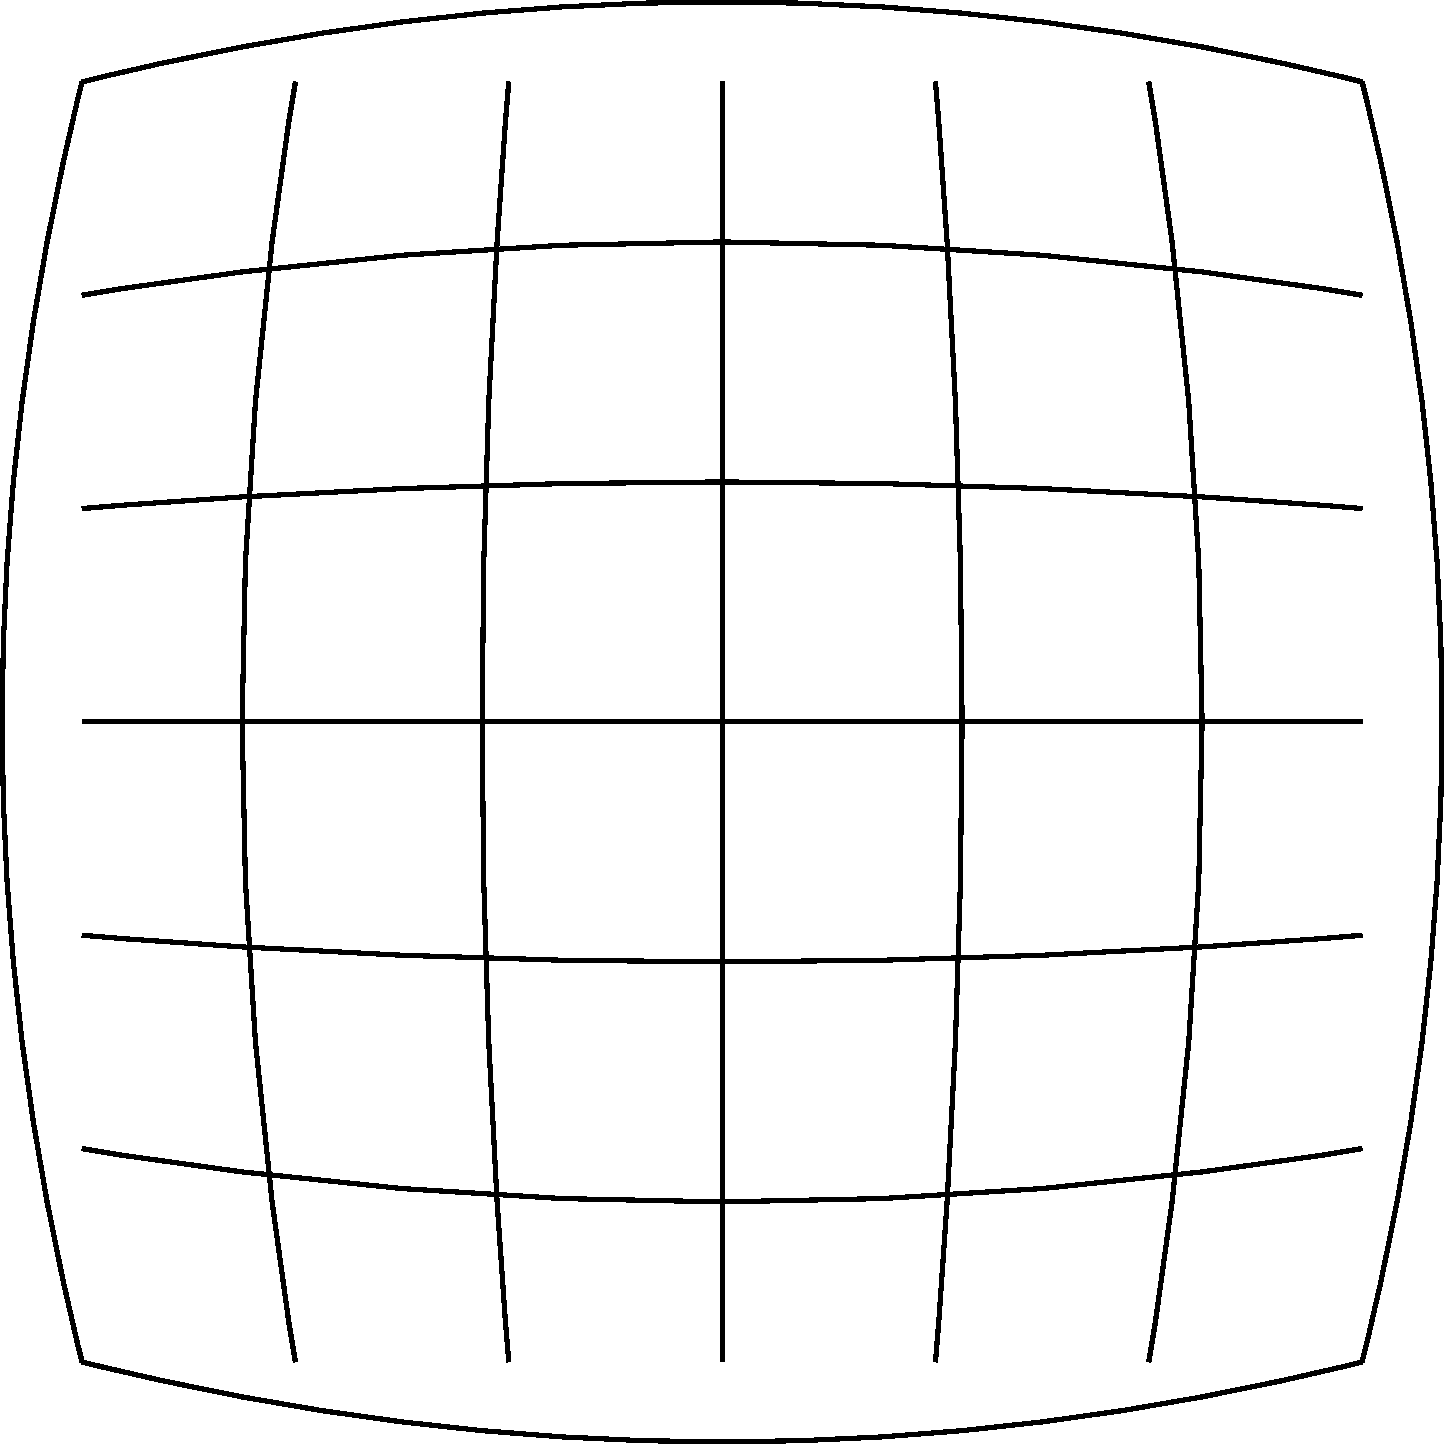
\includegraphics[width=0.25\textwidth]{gfx/barrel-distortion}}
		\hfill
		\subfloat[Simple lens system (Wikipedia/DrBob)]{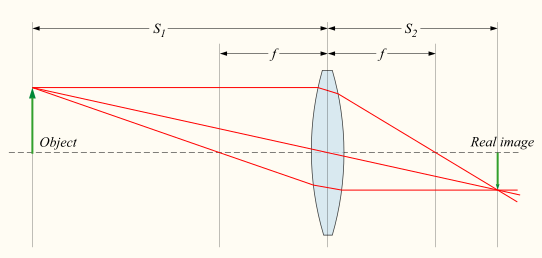
\includegraphics[width=0.70\textwidth]{gfx/lens3}}
		\hfill
	\end{figure}
		   	% \kuva{0.1}{barrel-distortion}

%\kuva{0.6}{lens3}
%{ \centering { \footnotesize Wikipedia/DrBob } \par }

\begin{itemize}
	\item Aperture size, depth of field, shutter speed, motion blur, diffraction, distortion, ...
	\item Capture hardware, image resolution, noise, frame rate, compression quality, ...
	\item Physical units, camera location, multi-camera calibration
\end{itemize}
\end{frame}

%%%%%%%%%%%%%%%%%%%%%%%%%%%%%%%%%%%%%%%%%%%%%%%%%%%%%%%%%%%%%%%%%%%%%%%%%%%%%%%%%%%%%%%%%%%%%

%\begin{frame}{Real cameras}
%\kuva{0.1}{barrel-distortion}
%\begin{align}
%	r &= \sqrt{(x - x_c)^2 + (y - y_c)^2}\\
%	x_{corr} &= x(1 + k_1 r^2 + k_2 r^4 + k_3 r^6)\\
%	y_{corr} &= y(1 + k_1 r^2 + k_2 r^4 + k_3 r^6)
%\end{align}
%Brown's distortion model (1966)
%%\kuva{0.6}{ankka.jpg}
%\end{frame}

%%%%%%%%%%%%%%%%%%%%%%%%%%%%%%%%%%%%%%%%%%%%%%%%%%%%%%%%%%%%%%%%%%%%%%%%%%%%%%%%%%%%%%%%%%%%%

\begin{frame}{Movies}
\simplefig{h!}{
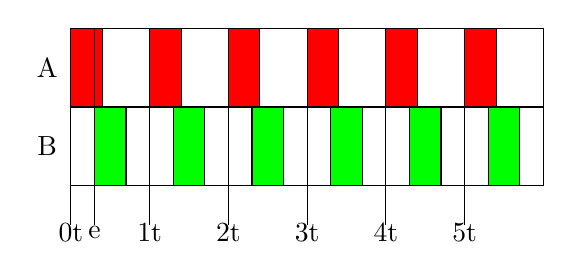
\begin{tikzpicture}[scale=1.0]]
	\draw (0,0) rectangle (6,-1);
	\draw (0,-1) rectangle (6,-2);
	\foreach \x in {0,...,5} {
		\draw (\x*1, 0) -- (\x*1, -2.5);
		\node at (\x*1, -2.6) {{\x}t};

		\draw [fill=red] (\x*1, 0) rectangle (\x*1+0.4, -1);
		\draw [fill=green] (\x*1+0.3, -1) rectangle (\x*1+0.3+0.4, -2);
	}
	\draw (0.3, 0) -- (0.3, -2.5);
	\node at (0.3, -2.6) {e};
	\node at (-0.3, -0.5) {A};
	\node at (-0.3, -1.5) {B};
	% P, Z
\end{tikzpicture}
}{fig:syncproblems}
{}
\begin{itemize}
	\item Motion blur
	\item Rolling shutter
	\item Sub-frame synchronization
	\item Other issues (23.57(6) FPS, mechanics, wiring, ..)
\end{itemize}
\end{frame}

%%%%%%%%%%%%%%%%%%%%%%%%%%%%%%%%%%%%%%%%%%%%%%%%%%%%%%%%%%%%%%%%%%%%%%%%%%%%%%%%%%%%%%%%%%%%%

\begin{frame}{Calibration, camera parameters}
	\begin{figure}
		\hfill
		\subfloat{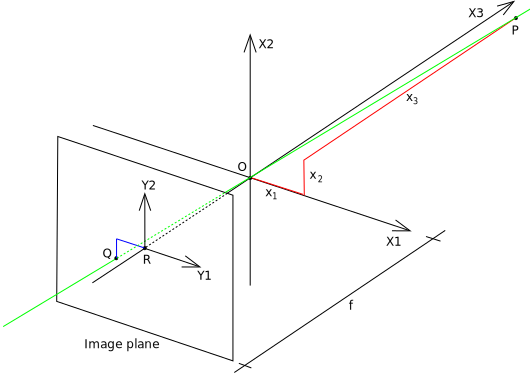
\includegraphics[width=0.45\textwidth]{gfx/pinhole3d}}
		\hfill
		\subfloat{$
	\begin{pmatrix}
		\alpha_x f & \gamma   & u_0\\
		0        & \alpha_y f & v_0\\
		0        & 0        & 1
	\end{pmatrix}
$}
		\hfill
	\end{figure}
\begin{itemize}
	\item Given known 3D coordinates and corresponding images, what is the projection matrix? (intrinsics, extrinsics)
	\item Done for single cameras and camera systems
	\item Projections closely related to computer graphics in general
\end{itemize}
%\kuva{0.6}{ankka.jpg}
\end{frame}

%%%%%%%%%%%%%%%%%%%%%%%%%%%%%%%%%%%%%%%%%%%%%%%%%%%%%%%%%%%%%%%%%%%%%%%%%%%%%%%%%%%%%%%%%%%%%

\begin{frame}{(Multi view) stereo}
\kuva{0.6}{stanford}
\centering Stanford camera array.

Several cameras imaging the same scene at the same time
\end{frame}

%%%%%%%%%%%%%%%%%%%%%%%%%%%%%%%%%%%%%%%%%%%%%%%%%%%%%%%%%%%%%%%%%%%%%%%%%%%%%%%%%%%%%%%%%%%%%

\begin{frame}{Disparity}
\simplefig{h!}{
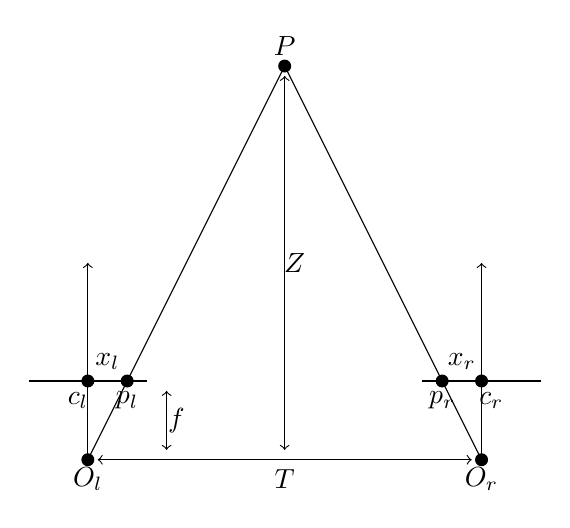
\begin{tikzpicture}[scale=0.25]
	% P, Z
	\draw[fill] (0, 20) circle [radius=0.3];
	\node at (0, 21) {$P$};

	\draw [<->] (0, 0.5) -- (0, 19.5);
	\node at (0.5, 10) {$Z$};

	% origins, T
	% TODO: circles, node ends not exactly at those points
	\draw [<->] (-9.5,0) -- (9.5, 0);
	\draw[fill] (-10, 0) circle [radius=0.3];
	\draw[fill] ( 10, 0) circle [radius=0.3];
	\node at (-10, -1) {$O_l$};
	\node at (10, -1) {$O_r$};
	\node at (0, -1) {$T$};

	% headings
	\draw [->] (-10, 0) -- (-10, 10);
	\draw [->] (10, 0) -- (10, 10);

	% image planes, at y=4
	\draw[thick] (-13, 4) -- (-7, 4);
	\draw[thick] (13, 4) -- (7, 4);

	\draw [<->] (-6, 0.5) -- (-6, 3.5);
	\node at (-5.5, 2) {$f$};


	% intersection points at principals and xs
	\draw[fill] (-10, 4) circle [radius=0.3];
	\draw[fill] (10, 4) circle [radius=0.3];

	\node at (-10.5, 3) {$c_l$};
	\node at (10.5, 3) {$c_r$};

	\node at (-9, 5) {$x_l$};
	\node at (9, 5) {$x_r$};


	% O-to-P
	\draw (-10, 0) -- (0, 20);
	\draw (10, 0) -- (0, 20);


	% p
	\draw[fill] (8, 4) circle [radius=0.3];
	\node at (8, 3) {$p_r$};
	\draw[fill] (-8, 4) circle [radius=0.3];
	\node at (-8, 3) {$p_l$};
\end{tikzpicture}
}{fig:simplestereo} {}

Two identical cameras; depth inversely related to $x_r - x_l$, i.e. pixel disparity between corresponding points in images

\end{frame}

%%%%%%%%%%%%%%%%%%%%%%%%%%%%%%%%%%%%%%%%%%%%%%%%%%%%%%%%%%%%%%%%%%%%%%%%%%%%%%%%%%%%%%%%%%%%%

\begin{frame}{Epipolar geometry}
\simplefig{h!}{
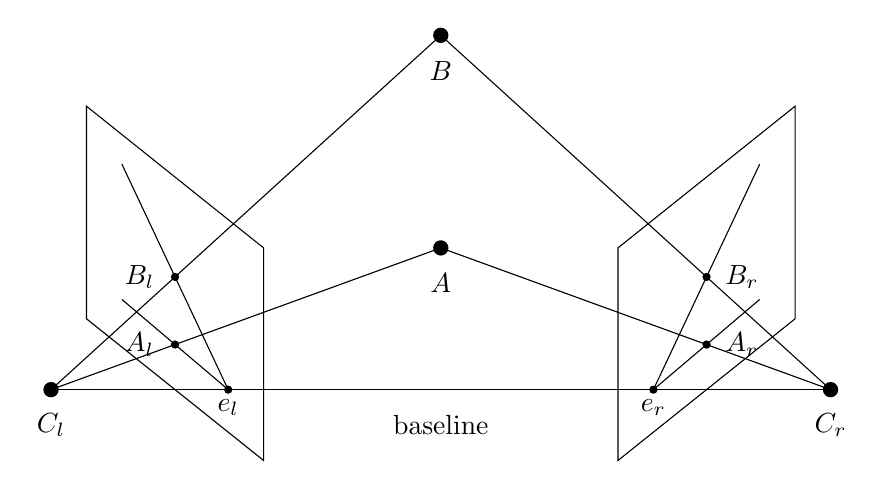
\begin{tikzpicture}[scale=0.45]
	% cameras
	\draw[fill] (-11,-1) circle [radius=0.2];
	\draw[fill] ( 11,-1) circle [radius=0.2];
	\draw (-11,-1) -- (11, -1);
	\node at (0, -2) { baseline };

	\node at (-11,-2) {$C_l$};
	\node at ( 11,-2) {$C_r$};

	% planes
	\draw (-10,1) -- (-10,7) -- (-5,3) -- (-5,-3) -- cycle;
	\draw ( 10,1) -- ( 10,7) -- ( 5,3) -- ( 5,-3) -- cycle;

	% 3d pts
	\draw[fill] ( 0,3) circle [radius=0.2];
	\draw[fill] ( 0,9) circle [radius=0.2];
	\node at (0,2) {$A$};
	\node at (0,8) {$B$};

	% origins via pts
	\draw (-11,-1) -- (0,3) -- (11,-1);
	\draw (-11,-1) -- (0,9) -- (11,-1);

	% epis
	\draw[fill] (-6,-1) circle [radius=0.1];
	\draw[fill] (6,-1) circle [radius=0.1];
	\node at (-6,-1.5) { $e_l$ };
	\node at (6,-1.5) { $e_r$ };

	% projections
	\draw[fill] (-7.5,0.2727) circle [radius=0.1];
	\draw[fill] (-7.5,2.1818) circle [radius=0.1];
	\node at (-8.5, 0.2727) {$A_l$};
	\node at (-8.5, 2.1818) {$B_l$};
	% lines from epis
	\draw (-6,-1) -- +(-2*1.5,2*1.2727);%(-7.5,0.2727);
	\draw (-6,-1) -- +(-2*1.5,2*3.1818);%(-7.5,2.1818);

	\draw[fill] (7.5,0.2727) circle [radius=0.1];
	\draw[fill] (7.5,2.1818) circle [radius=0.1];
	\node at (8.5, 0.2727) {$A_r$};
	\node at (8.5, 2.1818) {$B_r$};
	\draw (6,-1) -- +(2*1.5,2*1.2727);%(7.5,0.2727);
	\draw (6,-1) -- +(2*1.5,2*3.1818);%(7.5,2.1818);
\end{tikzpicture}
}{fig:epigeom} {}

Corresponding points are found on lines. Rectification twists the images so that those lines become horizontal (or vertical).
\end{frame}

%%%%%%%%%%%%%%%%%%%%%%%%%%%%%%%%%%%%%%%%%%%%%%%%%%%%%%%%%%%%%%%%%%%%%%%%%%%%%%%%%%%%%%%%%%%%%

\begin{frame}{Really multi-view}
\begin{itemize}
	\item Two camera case is still pretty dull
	\item Combine pairs, reconstruct individually, register in 3d
	\item Several on same baseline, match pairwise, fit least errors
	\item Use lots, arbitrarily positioned, magic algorithms
	\item Single camera traversing in a scene (SfM)
\end{itemize}
%\kuva{0.6}{ankka.jpg}
\end{frame}

%%%%%%%%%%%%%%%%%%%%%%%%%%%%%%%%%%%%%%%%%%%%%%%%%%%%%%%%%%%%%%%%%%%%%%%%%%%%%%%%%%%%%%%%%%%%%

\begin{frame}{From static to dynamic}
\begin{itemize}
	\item Static can be scanned with a single camera only
	\item Moving targets need static frames from many angles
	\item Images must be consistent within a frame
	\item Reconstruction (usually) for static objects
	\item Stream of static frames reconstructed, or more sophisticated tracking
\end{itemize}
%\kuva{0.6}{ankka.jpg}
\end{frame}

%%%%%%%%%%%%%%%%%%%%%%%%%%%%%%%%%%%%%%%%%%%%%%%%%%%%%%%%%%%%%%%%%%%%%%%%%%%%%%%%%%%%%%%%%%%%%

\begin{frame}{Dynamic methods}
\begin{itemize}
	\item Brute force reconstruction of every video frame
	\item Register together, build a mesh while going
	\item Morph initial model based on frame deformations
	\item Track local pre-selected features in 2D
	\item Track features in 3D, deform mesh based on keypoints
	\item And more and more post-processing
\end{itemize}
%\kuva{0.6}{ankka.jpg}
\end{frame}

%%%%%%%%%%%%%%%%%%%%%%%%%%%%%%%%%%%%%%%%%%%%%%%%%%%%%%%%%%%%%%%%%%%%%%%%%%%%%%%%%%%%%%%%%%%%%

\begin{frame}{Post process}
\begin{itemize}
	\item Actually, assumptions on the object often used
	\item Initial scan of an object, rest model
	\item Sometimes features tracked in 2D or 3D (still pre-recorded)
	\item Feature spaces and parameterizations in extreme cases
\end{itemize}
%\kuva{0.6}{ankka.jpg}
\end{frame}

%%%%%%%%%%%%%%%%%%%%%%%%%%%%%%%%%%%%%%%%%%%%%%%%%%%%%%%%%%%%%%%%%%%%%%%%%%%%%%%%%%%%%%%%%%%%%]

\begin{frame}{Texture and topology}
\begin{itemize}
	\item Reconstruction outputs local geometry properties
	\item Color per vertex, not textured, not meshed
	\item Reconstruct surface topology: fit data to surface, fill holes; use models
	\item Reproject camera views on ready mesh to recover texture maps
	\item Sometimes features tracked in 2D or 3D (still pre-recorded)
	\item Feature spaces and parameterizations in extreme cases
\end{itemize}
%\kuva{0.6}{ankka.jpg}
\end{frame}

%%%%%%%%%%%%%%%%%%%%%%%%%%%%%%%%%%%%%%%%%%%%%%%%%%%%%%%%%%%%%%%%%%%%%%%%%%%%%%%%%%%%%%%%%%%%%

\begin{frame}{In practice}
\kuva{0.6}{fifa}
\centering { \small (EA sports, FIFA '14; 18 DSLRs) }
\begin{itemize}
	\item Shutter delay and jitter, flash sync, remote control
	\item construction, calibration convenience, bad software,
	\item Manual work, 3D noise removal, artist work, magic coefficients
\end{itemize}
\end{frame}

%%%%%%%%%%%%%%%%%%%%%%%%%%%%%%%%%%%%%%%%%%%%%%%%%%%%%%%%%%%%%%%%%%%%%%%%%%%%%%%%%%%%%%%%%%%%%

\begin{frame}{Still software}
\begin{itemize}
	\item Libs: OpenCV, Point Cloud Library, Computational Geometry Algorithms Library, ...
	\item Free: Camera calibration toolbox for Matlab (+OpenCV), Bundler, Sift, SiftGPU, PBA, PMVS/CMVS, VisualSFM, Meshlab, PoissonRecon, CmpMVS, Python photogrammetry toolbox, ...
	\item Commercial: Photosynth, 123D Catch, Agisoft PhotoScan, CaptiveMotion, MotionScan, Faceshift, 3DF Zephyr Pro, Mova Contour Reality Capture, Pendulum Studio, Pix4DMapper, Acute3D, ...
\end{itemize}
%\kuva{0.6}{ankka.jpg}
\end{frame}

%%%%%%%%%%%%%%%%%%%%%%%%%%%%%%%%%%%%%%%%%%%%%%%%%%%%%%%%%%%%%%%%%%%%%%%%%%%%%%%%%%%%%%%%%%%%%

\begin{frame}{VisualFSM}
	\kuva{0.8}{visualsfm}
\end{frame}

%%%%%%%%%%%%%%%%%%%%%%%%%%%%%%%%%%%%%%%%%%%%%%%%%%%%%%%%%%%%%%%%%%%%%%%%%%%%%%%%%%%%%%%%%%%%%

\begin{frame}{Meshlab}
	\kuva{0.8}{meshlab}
\end{frame}

%%%%%%%%%%%%%%%%%%%%%%%%%%%%%%%%%%%%%%%%%%%%%%%%%%%%%%%%%%%%%%%%%%%%%%%%%%%%%%%%%%%%%%%%%%%%%

\begin{frame}{Meshlab}
	\kuva{0.8}{meshlab2}
\end{frame}

%%%%%%%%%%%%%%%%%%%%%%%%%%%%%%%%%%%%%%%%%%%%%%%%%%%%%%%%%%%%%%%%%%%%%%%%%%%%%%%%%%%%%%%%%%%%%

\begin{frame}{Meshlab}
	\kuva{0.8}{meshlab3}
\end{frame}

%%%%%%%%%%%%%%%%%%%%%%%%%%%%%%%%%%%%%%%%%%%%%%%%%%%%%%%%%%%%%%%%%%%%%%%%%%%%%%%%%%%%%%%%%%%%%

\begin{frame}{Conclusion}
\begin{itemize}
	\item Multi-step pipeline from construction to shooting, reconstruction and post-processing
	\item Used method(s) largely application specific
	\item Lots of software, special applications coming, rising trend
	\item MVS just one scanning method
\end{itemize}
Many tools integrate some steps or add in their own
%\kuva{0.6}{ankka.jpg}
\end{frame}


%%%%%%%%%%%%%%%%%%%%%%%%%%%%%%%%%%%%%%%%%%%%%%%%%%%%%%%%%%%%%%%%%%%%%%%%%%%%%%%%%%%%%%%%%%%%%

\end{document}
